\documentclass[a4paper,parskip=half]{article} %scrartcl

\bibliographystyle{alpha}

\usepackage[utf8]{inputenc}
\usepackage[T1]{fontenc}
\usepackage{amsmath,mathtools,amssymb,listingsutf8,xspace}
\usepackage{geometry,hyperref,cleveref,xcolor}
\usepackage[disable]{todonotes}
\usepackage{tikz-cd}

\usetikzlibrary{positioning}

\newcommand*\cmdstyle\texttt
\newcommand*\file\cmdstyle
\newcommand*\literalColor{blue}
\newcommand*\cmd[1]{\cmdstyle{\textcolor{red!85!black}{#1}}}
\newcommand*\cmdline[1]{\cmdstyle{\textcolor{green!70!black}\$ }\cmd{#1}}
\newcommand*\literal[1]{\textcolor{\literalColor}{\cmdstyle{#1}}}
\newcommand*\api[1]{\textcolor{purple}{\cmdstyle{#1}}}
\newenvironment{cmdhelp}{\begin{quote}\footnotesize}{\end{quote}}


\newcommand\removed[1]{}
%\newcommand\added[1]{{\color{green!70!black}#1}}
\newcommand\added[1]{#1}
\newcommand\changedto[2]{%
    \removed{#1}%
    \added{#2}}
\newcommand\changed[1]{{\color{blue}#1}}

\newcommand*\eqdef=


\newcommand*\dom{\operatorname{dom}}
\newcommand*\range{\operatorname{range}}
\newcommand*\query{\operatorname{\mathsf{query}}}
\newcommand*\assert{\operatorname{\mathsf{assert}}}
\newcommand*\rad{\operatorname{rad}}
\newcommand*\regmin[2]{\llfloor{#1}\rrfloor_{#2}}
%\newcommand*\regmax[2]{\llceil{#1}\rrceil_{#2}}
\newcommand*\regmax[2]{[[{#1}]]_{#2}}
%\newcommand*\objv{\operatorname{objv}}
\newcommand*\objv{o}




\newcommand*\Solver{Symbolic Machine Learning Prover\xspace}
\newcommand*\SolverAbbrvText{SMLP}
\newcommand*\SolverAbbrv{\SolverAbbrvText\xspace}
\newcommand*\SolverVersion{v0.1}

\newcommand*\progmrc{smlp-mrc.sh}
\newcommand*\provenn{prove-nn.py}
\newcommand*\trainnn{train-nn.py}

\newcommand*\todofb[2][]{\todo[color=cyan!30,tickmarkheight=.2em,size=\scriptsize,#1]{FB: #2}}
%\newcommand*\todozk[2][]{\todo[color=yellow!30,tickmarkheight=.2em,size=\scriptsize,#1]{ZK: #2}}
\newcommand\todozk[1]{\textcolor{red}{#1}}
%\newcommand*{\todozk}[2][1=]{\todo[linecolor=red,backgroundcolor=red!25,bordercolor=red,#1]{#2}}
\newcommand*\todokk[2][]{\todo[color=purple!20,tickmarkheight=.2em,size=\scriptsize,#1]{KK: #2}}


\newtheorem{thm}{Theorem} %[section]
\newtheorem{lem}[thm]{Lemma}
\newtheorem{conj}[thm]{Conjecture}
\newtheorem{prop}[thm]{Proposition}
\newtheorem{defn}[thm]{Definition}


\newcommand*\KK{\todokk}
\newcommand*\ZK{\todozk}
\newcommand{\delete}[1]{}

\title{The \Solver}
\author{%
	Franz Brauße \and
	Zurab Khasidashvili \and
	Konstantin Korovin
}

\begin{document}
\maketitle
\begin{abstract}


\Solver (\SolverAbbrv) is a collection of tools for reasoning about machine
learning models. \SolverAbbrv is based on SMT solver(s). In this document we
describe functionality for computing safe and stable regions of neural network
models satisfying optput specifications. This corresponds to solving
$\epsilon$-guarded $\exists^*\forall^*$ formulas over NN
representations~\cite{BKK20}.

%\Solver (\SolverAbbrv) is a distribution of tools around an SMT-based solver for
%computing safety thresholds of functions defined by NNs on regions in bounded
%domains. At its core are the algorithms for solving $\epsilon$-guarded
%$\exists^*\forall^*$ formulas~\cite{BKK20}.

\SolverAbbrv has been developed by
\href{mailto:brausse@informatik.uni-trier.de?subject=\SolverAbbrvText}{Franz Brauße},
Zurab Khasidashvili
and Konstantin Korovin and is available
under the terms of the Apache License v2.0.%
\footnote{\url{https://www.apache.org/licenses/LICENSE-2.0}}
\end{abstract}
\tableofcontents

\section{Changes}
\begin{itemize}
\item 07/07/2020: documentation of \SolverAbbrv v0.1
\end{itemize}

\section{Introduction}

\emph{Symbolic Machine Learning Prover} (SMLP) offers multiple capabilities for system's \emph{design space exploration}.
These capabilities include methods for selecting which parameters to use in modeling design for configuration optimization and verification;
ensuring that the design is robust against environmental effects and manufacturing variations that are impossible to control, as well as ensuring 
robustness against malicious attacks from an adversary aiming at altering the intended configuration or mode of operation.
Environmental affects like temperature fluctuation, electromagnetic interference, manufacturing variation, and product aging effects are especially 
more critical for correct and optimal operation of devices with analog components, which is currently the main focus area for applying  SMLP.

To address these challenges, SMLP offers multiple modes of design space exploration; they will be discussed in detail in Section~\ref{sec:exploration}.
The definition of these modes refers to the concept of \emph{stability} of an assignment to system's parameters that satisfies all model constraints 
(which include the constraints defining the model itself and any constraint on model's interface).
We will refer to such a value assignment as a \emph{stable witness}, or \emph{(stable) solution} satisfying the model constraints. 
Informally, stability of a solution means that any eligible assignment in the specified region around the solution also satisfy the required constraints.
This notion is sometimes referred to as robustness. We work with parameterized systems, where parameters (also called \emph{knobs}) can 
be tuned to optimize the system's performance under all legitimate inputs.
For example, in the circuit board design setting, topological layout of circuits, distances, wire thickness, properties of dielectric layers, etc.
can be such parameters, and the exploration goal would be to optimize the system performance under the system's requirements~\cite{9501615}.
The difference between knobs and inputs is that knob values are selected during design phase, before the system goes into operation; on the other hand, 
inputs remain free and get values from the environment during the operation of the system. Knobs and inputs correspond to existentially quantified 
and universally quantified variables in the formal definition of model exploration tasks. Thus in the usual meaning of verification, optimization and synthesis, 
respectively, all variables are inputs, all variables are knobs, and some of the variables are knobs and the rest are inputs.


Below by a \emph{model} we refer to an ML model that models the system under exploration.

\ZK{Could not used column sep = {8.5em, between origins} option in the cube.}
\begin{figure}[bp] %column sep = {8.5em, between origins}
\centering
\[
    \begin{tikzcd}[row sep=1.5em, column sep = {8.5em}, my label/.style={midway, sloped}]
    \bullet
    \arrow[rr, "\text{stable-optimization}"]
    \arrow[dr, swap,"\text{stable-synthesis}"{anchor=north,rotate=-18}]
    &&
    \bullet
    \arrow[dr]
    \\
    &
    \bullet
    \arrow[rr]
    &&
    \bullet
    \\
    \bullet
    \arrow[uu, "\text{stability}"{anchor=north,rotate=90}] 
    \arrow[rr, dashed, "\text{optimization}"] 
    \arrow[dr, swap, "\text{synthesis}"{anchor=south, rotate=-18}] 
    \arrow[rrru, dashdotted, "\text{stable optimized synthesis}"{anchor=south, rotate=6}]
    &&
    \bullet  
    \arrow[dr, dashed] 
    \arrow[uu, dashed]
    \\
    &
    \bullet
    \arrow[rr] 
    \arrow[uu]
    && 
    \bullet
    \arrow[uu]
    \end{tikzcd}
\]
\caption{Exploration Cube}
\label{fig:cube}
\end{figure}

The \emph{model exploration cube} in Figure~\ref{fig:cube} provides a high level and intuitive idea on how the model exploration modes supported in SMLP are related.
The three dimensions in this cube represent synthesis ($\searrow$-axis), optimization ($\rightarrow$-axis) and stability ($\uparrow$-axis).
On the bottom plane of the cube, the edges represent the synthesis and optimization problems in the following sense:
synthesis with constraints configures the knob values in a way that guarantees that assertions are valid, but unlike optimization, does not guarantee optimally with respect to optimization objectives.
%\changed%
%\todofb{yet, optimization is not aware of assertions on inputs and thus its results are not guaranteed to be valid in the configured system by itself}%
%while optimization guarantees near-optimality \todozk{near-optimality...; also drop ''(in a precise sense)''} (in a precise sense) with respect to optimization objectives but is not aware of assertions on inputs thus cannot guarantee their validity in the configured system.
We refer to the process that combines synthesis with optimization and results in an optimal design that satisfies assertions as \emph{optimized synthesis}.
The upper plane of the cube represents introducing stability requirements into synthesis (and as a special case, into verification), optimization, and optimized synthesis.
The formulas that make definition of stable verification, optimization, synthesis and optimized synthesis precise are discussed in \changedto{Section~\ref{sect.exploration}}{Sections~\ref{sect.exploration} to \ref{sec:expl}}.

\section{Concepts and Preliminaries}
In this document, syntactical highlights are placed on
\literal{literal strings}, which are ASCII sequences used to communicate input
to and output from programs; on \cmd{commands} to be executed;
and on \api{API references} which correspond to
either concrete symbols or abstract concepts defined in the corresponding API.

We assume familiarity with JSON, \cmd{make} and CSV files. Since the CSV format
is not unambiguously defined, we give the concrete requirements in
\cref{sec:csv}.

The glossary in this section defines concepts which are used throughout this
document when describing in detail the problems solved by \SolverAbbrv and is
meant to be referred to on an per-instance basis instead of reading it as a
whole.
\begin{description}
\item[Center Threshold]
	A rational value in $[0,1]$ larger or equal to Threshold.
\item[Codomain]
	A real vector space.
\item[Data set]
	A list of points in $D\times C$ where $D$ is the domain and $C$ is the
	codomain.
\item[Domain]
	A domain $D$ is the cartesian product $\bigtimes_{i=1}^n D_i$ where
	$D_i$ is a subset of either $\mathbb Z$, $\mathbb R$ or a
	discrete finite subset of $\mathbb Q$.
\item[Feature]
	Any column of a data set $\mathcal D$ is called a feature.
\item[Instance]
	A tuple
	$(N,\mathcal N_D,o,\mathcal N_o)$ is called an instance if
	$N$ is an NN over domain $D$, $\mathcal N_D$ is a data normalization,
	$o$ is an objective function and
	$\mathcal N_O$ is an objective normalization.
	If -- in addition to an instance $I$ -- a data set $\mathcal D$ over $D$
	is given, $(I,\mathcal D)$ is called a data instance.
\item[NN]
	Neural network as understood by the Keras API of Tensorflow in HDF5
	format.
	In particular, the \Solver only handles \api{Dense} layers with either
	\api{relu} or \api{linear} activation function.
	The input layer must be defined on domain $D$ and the output layer
	must map to the codomain $C$.
\item[Region]
	Given a domain $D=\bigtimes_{i=1}^d D_i$, a region (in $D$) is a
	product $\bigtimes_{i=1}^d C_i$ where
	each $C_i\subseteq D_i$ is a finite union of compact intervals for
	$i=1,\ldots,n$.
	For discrete $D_i$, e.g., a subset of $\mathbb Z$,
	$C_i$ is the finite union of point intervals.
	Otherwise, $D_i$ is a bounded subset of $\mathbb R$ and $C_i$
	corresponds to just one interval $[c_i\pm r_i]$ with center $c_i\in D_i$
	and rational radius $r_i>0$.
\item[Safe]
	A region $R$ is considered safe (wrt.\ a given target function $f$) for a
	constant $t\in\mathbb Q$ if $f$ satisfies $f(x)\geq t$
	for all $x\in R$.
\item[.spec]
	Specification file describing the domain, codomain and regions in the
	domain. Its format is a JSON list where the $i$-th entry corresponds to
	the $i$-th column in the CSV describing the data set.

	Given a data set and a .spec file, the components $D_i$ of the domain
	are defined as $D_i=E_i(F_i)$ where
	$E_i$ is called the embedding of $F_i$ into $D_i$ where $F_i$ is the
	$i$-th input feature.
%\item[Stable]
\item[Target function]
	The target function $f_I$ of an instance
	$I=(N,\mathcal N_D,o,\mathcal N_o)$ is defined as the composition
	$\mathcal N_o\circ o\circ\mathcal N_{D,\mathrm o}\circ
	N\circ\mathcal N_{D,\mathrm i}$.
	The target function $f_{I,\mathcal D}$ of a data instance
	$(I,\mathcal D)$ is
	$x\mapsto\min(\{f_I(x)\}\cup\{\mathcal N_o(o(y)):(x,y)\in\mathcal D\})$.
\item[Threshold]
	The threshold for a region $R$ and target function $f$ is defined
	as the maximal $t\in\{t_1,\ldots,t_n\}\subset[0,1]\cap\mathbb Q$ for
	which $R$ is safe wrt.\ $f$ for $t$ if it exists, and $-\infty$ otherwise.

	The threshold for a domain $D$ and target function $f$ is defined
	as the maximal $t\in\{t_1,\ldots,t_n\}\subset[0,1]\cap\mathbb Q$ for
	which there is a region that is safe wrt.\ $f$ for $t$ if it exists, and
	$-\infty$ otherwise.
\end{description}

%\section{Overview}



\section{Prerequisites}
This section describes software environments \SolverAbbrv is known to work in.
All packages corresponding to software listed in in \Cref{list:libs} should be
installed ``system-wide'',
meaning that they are accessible to the corresponding interpreter or compiler
listed in \Cref{list:comp-int} without additional options.

Please note, that \SolverAbbrv may run with versions of the packages not listed
here. These lists are subject to change and are gradually extended as soon as
more versions have been tested or other package requirements arise.

\subsection{Compilers / Interpreters / Utils}\label{list:comp-int}
These tools should be available in one of the paths
mentioned in the \texttt{PATH} environment variable.
\begin{itemize}
\item \cmd{bash}: GNU Bourne Again Shell version 5.0\_p17
	\url{http://tiswww.case.edu/php/chet/bash/bashtop.html}
\item \cmd{gmake}: GNU make version 4.1, 4.2 or 4.3
	\url{https://www.gnu.org/software/make/make.html}
\item \cmd{awk}: GNU awk version 5.0.1 or 5.1
	\url{https://www.gnu.org/software/gawk/gawk.html}
\item \cmd{sed}: GNU sed version 4.8
	\url{http://sed.sourceforge.net/}
\item GNU coreutils version 8.32
	\url{https://www.gnu.org/software/coreutils/}
\item GNU time version 1.7, 1.7.2 or 1.9
	\url{https://www.gnu.org/directory/time.html}
\item \cmd{cc}: either GNU C Compiler version 4.7.4, 5.4.0, 9.3.0 or 10.1.0
	\url{https://gcc.gnu.org/}
	or Clang version 10.0.0
	\url{https://clang.llvm.org/}
\item \cmd{python3}: CPython version 3.6 or 3.7
	\url{https://www.python.org/}
\end{itemize}

\subsection{Libraries}\label{list:libs}
The paths to the installed \texttt{python} directory should be set in the
\texttt{PYTHONPATH} environment variable. See \cmd{python3 -h} for details on
this variable.
\begin{itemize}
\item Tensorflow version 2.1 or 2.2 \url{https://www.tensorflow.org/}
\item Z3 including its Python API version 4.8.6 or 4.8.8
	\url{https://github.com/Z3Prover/z3}
\item Pandas version 0.24.2 \url{https://pandas.pydata.org/}
\item scikit-learn version 0.20.4 or 0.22.2\_p1
	\url{https://scikit-learn.org/}
\item matplotlib version 2.2.4 or 3.1.2
	\url{https://matplotlib.org/}
\item seaborn version 0.9.x or 0.10.x
	\url{https://seaborn.pydata.org/}
\item HDF5 for Python version 2.10.0
	\url{https://www.h5py.org/}
\item kjson version 0.1.3 (bundled in release)
	\url{https://github.com/fbrausse/kjson}
\end{itemize}


\section{Training ML models with SMLP}\label{sec:models}

SMLP supports training tree-based and polynomial models using the scikit-learn\footnote{\url{https://scikit-learn.org/stable/}} 
and pycaret\footnote{\url{https://pycaret.org}} packages, 
and training neural networks using the Keras package with TensorFlow\footnote{\url{https://keras.io}}. 
For systems with multiple outputs, SMLP supports training one model with multiple outputs as well as training separate models per response 
(this is controlled by command-line option $model\_per\_response$). Supporting these two options allows a trade-off between the accuracy 
of the models (models trained per response are likely to be more accurate) and with the size of the formulas that represent the model for 
symbolic analysis (one multi-output model formula will be at least smaller when the same training hyper-parameters are used). 
Conversion of models to formulas into SMLP language is done internally in SMLP (no encoding options are exposed to user in current 
implementation, which will change once alternative encodings will be developed).



\section{ML model exploration with SMLP}\label{sec:exploration}

SMLP supports the following model exploration modes (we assume that an ML model $M$ has already been trained). 
\begin{itemize}
\item[certify] Given an ML model $M$, a value assignment $a$ to knobs, and a query $\query$, check that $a$ is a stable 
witness for $\query$ on model $M$. Multiple pairs $(a,\query)$ of candidate witness $a$ and query $\query$ can be checked in a single SMLP run.
\item[query] Given an ML model $M$  and a query $\query$, find a stable witness $a$  for $\query$ on $M$.
\item[verify] Given an ML model $M$,  a value assignment $a$ to knobs,  and an assertion $\assert$, verify whether  
$\assert$ is valid on model $M$ for any legal inputs (for the given value assignment $a$ to knobs). SMLP supports verifying 
multiple assertions in a single run.
\item[synthesize] Given an ML model $M$,  find a stable configuration of knobs (a value assignment $a$ to knobs) 
such that required constraints (possibly including assertions),  are valid for all legal value assignments to the inputs.
\item[optimize]  Given an ML model $M$,  find a stable configuration of knobs that yields a pareto-optimal values of 
the optimization objectives (pareto-optimal with respect to the \emph{max-min} optimization problem defined in~\cite{BKK24}).
\item[optsyn] Given an ML model $M$,  find a stable configuration of knobs that yields a pareto-optimal values of the 
optimization objectives and all constraints and assertions are valid for all legal values of inputs. This mode is a union 
of the \emph{optimize} and \emph{synthesize} modes, its full name is \emph{optimized synthesis}. 
All the previous modes can be seen as a special case of optimized synthesis mode.
\end{itemize}

A formal definition of the tasks accomplished with these model exploration modes can be found in~\cite{BKK24}. 
Formal descriptions combined with informal clarifications will be provided in this section as well. 
Running SMLP in these modes reduces to solving formulas of the following structure:
\begin{equation}\label{form:gear:final}
    \exists p ~\big[ \eta(p) \wedge
    \forall p'~
    \forall x y~[
    \theta(p,p') \implies (\varphi_M(p',x,y)  \implies  \varphi_{\mathit{cond}}(p',x,y))
    ]\big]
\end{equation}
where $p$ denotes model knobs, $x$ denotes inputs, $y$ denotes the outputs, $\eta(p)$ defines 
constraints on the knobs,  $\varphi_M(p',x,y)$ defines the ML model constraints, and the 
condition $\varphi_{\mathit{cond}}(p',x,y)$ depends on the SMLP mode and will discussed in subsections below.
In~\cref{form:gear:final}, $\theta(p,p')$ is in general a reflexive predicate, and in SMLP it is used as 
$\theta_r(p, p') \eqdef \Vert p - p' \Vert \leq r$, where  $\Vert p - p' \Vert$ is a distance between 
two configurations $p$ and $p'$, and $r$ is a relative or absolute \emph{radius}.


\begin{defn}\label{def:stable:witness:validity}
\begin{itemize}
\item Given a value assignment $p^*$ to knobs $p$, an assignment $x^*$ to inputs $x$ is called a \emph{$\theta$-stable witness} 
to $\query(p,x,y)$ for configuration $p^*$ if the following formula is valid:
\begin{equation}\label{form:gear:certify:knobs:inputs}
\varphi_{\mathit{witn}}^{px}(p^*,x^*) \eqdef
     \eta(p^*) \wedge ~\big(
    \forall p'~
    \forall y~[
   \theta(p^*, p') \implies (\varphi_M(p',x^*,y)  \implies  \varphi_{\mathit{cond}}(p',x^*,y))
    ]\big)
\end{equation}
where \[\varphi_{\mathit{cond}}(p,x,y) \eqdef \alpha(p,x) \implies \query(p,x,y).\]
In this case the value assignment $p^*, x^*$ to inputs and knobs $p,x$ is called a  \emph{$\theta$-stable witness for $\query(p,x,y)$}, 
and $x^*$ is called a  \emph{$\theta$-stable witness to $\query(p^*,x,y)$}.
\item A value assignment $p^*$ to knobs $p$ is called a  \emph{$\theta$-stable witness for $\query(p,x,y)$} if any legal value assignment 
$x^*$ to inputs $x$ is a $\theta$-stable witness to $\query(p,x,y)$ for $p^*$; that is, when the following formula is valid:
\begin{equation}\label{form:gear:certify:knobs}
\varphi_{\mathit{witn}}^{p}(p^*) \eqdef
     \eta(p^*) \wedge ~\big(
    \forall p'~
    \forall xy~[
   \theta(p^*, p') \implies (\varphi_M(p',x,y)  \implies  \varphi_{\mathit{cond}}(p',x,y))
    ]\big)
\end{equation}
\item An assertion $\assert(p, x,y)$ is called \emph{$\theta$-valid with respect to knob configuration $p^*$} if its negation 
$\query(p, x,y) \eqdef \neg \assert(p, x,y)$ does not have a $\theta$-stable witness $x^*$ for $p^*$.  In the latter case  
assertion $\assert(p^*, x,y)$ is called \emph{$\theta$-valid}. Otherwise, if $x^*$ is a  $\theta$-stable witness for 
$\query(p^*, x,y)$, then we call $x^*$  a \emph{$\theta$-stable counter-example to  $\assert(p^*, x,y)$}, and 
$\assert(p^*, x,y)$ is \emph{$\theta$-falsifiable} (that is, it is not $\theta$-valid).
\end{itemize}
\end{defn}


The idea behind the concept of $\theta$-validity of an assertion $\assert(p, x,y)$ with respect to a knob configuration $p^*$ is as follows. 
Under the assumption that the system is 
in one of the points in the $\theta$-stability region of $p^*$,  while the probability for the system of being in one of these points is $1$ 
(due to the assumption), the probability for the system of being in a particular point $x^*$ in the $\theta$-stability region is $0$.
\footnote{Here we have the situation that an infinite sun of $0$s is $1$. The number $1$ is selected because we are talking 
about probability and $1$ is the maximum probability. Here we want to make connection between stability and probability,
and we need an arithmetic / a calculus where an infinite sum of $0$s is not $0$. More precisely, likely we want $0 \times \aleph_0 = 0;\,\,
0 \times \aleph_1 = 1; \,\, \ldots ; \,\, 0 \times \aleph_i =  \aleph_{i-1} $ ($0$ times the cardinality of rationals;
 $0$ times the cardinality of reals, etc.).  Need to figure out what this calculus 
is -- maybe something related to the \emph{Uncertainty Principle} in quantum mechanics.} 
Now, consider  an input assignment $x^*$ such that $\query(p^*, x^*,y) \eqdef \neg \assert(p^*, x^*,y)$  holds and $x^*$ is not
a  $\theta$-stable witness to $\query(p^*,x,y)$. Then $x^*$ is a counter-example to $\assert(p^*, x, y)$, but $x^*$ can occur with probability $0$; 
%This means that when an input assignment $x^*$, such that $\query(p^*, x^*,y) \eqdef \neg \assert(p^*, x^*,y)$  holds, 
%is not a  $\theta$-stable witness to $\query$ for $p^*$,  $x^*$ is a counter-example  to $\assert$ but can happen with probability $0$; 
as a consequence, $\assert(p^*, x, y)$ does not have a counter-example with probability greater than $0$ and is therefore defined 
as $\theta$-valid in the above definition.




\subsection{Certification of candidate stable witness}\label{sect:certify}



Certification is defined both for a candidate stable configuration $p^*$ as well as for an assignment $p^*, x^*$ to both inputs and knobs.
\ZK{Still for now perturbation is defined for knobs only, not for inputs. Extension of perturbation to inputs requires more discussion (is this really needed?)}
Let's first consider the former case.
We are given a candidate configuration of knobs $p^*$ (which is a value assignment to knobs $p$), and a query $\query$ on an 
ML model $M$, and we want to check whether $p^*$ is a stable witness for $\query$. Intuitively, the latter means that $p^*$
satisfies $\query$ on model $M$ for any legal values of inputs $x$, even if the knob values in configuration $p^*$ are perturbed 
within a predefined radius. Formally, SMLP checks the validity of formula $\varphi_{\mathit{cert}}(p^*)$: 



\begin{equation}\label{form:gear:certify}
\varphi_{\mathit{cert}}(p^*) \eqdef
     \eta(p^*) \wedge ~\big(
    \forall p'~
    \forall x y~[
   \theta(p^*, p') \implies (\varphi_M(p',x,y)  \implies  \varphi_{\mathit{cond}}(p',x,y))
    ]\big)
\end{equation}

where \[\varphi_{\mathit{cond}}(p,x,y) \eqdef \alpha(p,x) \implies \query(p,x,y).\]
\noindent and  $\alpha(p,x)$ defines user-given constraints on knobs and inputs. 


For the above formula to be valid and not be valid vacuously, we need to check that $\eta(p^*)$ evaluates to constant true 
and  $\alpha(p^*,x)$ is satisfiable. This means that $p^*$ witnesses that $\alpha(p,x) \wedge \eta(p)$ is \emph{consistent}, 
that is, there exist values of inputs that satisfy  $\alpha(p^*,x) \wedge \eta(p^*)$. Formally, consistency check for stable 
witness certification requires the following formula to be valid: 

\begin{equation}\label{form:gear:certify:consistency}
\exists x~ [\alpha(p^*, x) \wedge \eta(p^*)])
\end{equation}


Syntactic checks in SMLP imposed on the specification file ensure that all knobs are assigned fixed values in $p^*$.  
If the consistency check fails, SMLP reports the status of $p^*$ as \emph{not a witness}; otherwise SMLP checks satisfiability 
of the following formula, which we refer to as \emph{feasibility} part of stable witness certification:

\begin{equation}\label{form:gear:certify:feasibility}
       \varphi_M(p^*,x,y)  \wedge  \alpha(p^*,x) \wedge   \query(p^*,x,y))
\end{equation}

If the above formula is not satisfiable, then $p^*$ cannot be a stable witness to $\query$, and SMLP reports its status as \emph{not a witness}. 
Otherwise stability of the candidate witness $p^*$ for $\query$ is checked by proving validity of formula \cref{form:gear:certify},
and this is done by checking satisfiability of formula~\cref{form:gear:certify:candidate}, which is the negation of the right conjunct of \cref{form:gear:certify}:
\begin{equation}\label{form:gear:certify:candidate}
     \theta(p^*, p')  \wedge  \varphi_M(p^*,x,y)  \wedge  \alpha(p^*,x) \wedge   \neg \query(p^*,x,y))
\end{equation}


SMLP supports checking multiple witness-query pairs in a single run. The status of each witness is reported in file 
 $prefix\_dataname\_certify\_results.json$, and each witness has one of these three status options:   
\begin{itemize}
\item \emph{not a witness} --formula ~\cref{form:gear:certify:consistency} is not valid or formula~\cref{form:gear:certify:feasibility} is not satisfiable.  
\item \emph{witness, not stable} -- formula~\cref{form:gear:certify} is not valid 
(formula~\cref{form:gear:certify:consistency} might still be valid and  formula~\cref{form:gear:certify:feasibility} satisfiable).
\item \emph{stable witness} -- formula~\cref{form:gear:certify} is valid (formula~\cref{form:gear:certify:candidate} is not satisfiable).
\end{itemize}

A results file might look like one on figure~\cref{fig:certify:result}:

\begin{figure}
\small
\begin{verbatim}
{
        "query1": "not a witness",
        "query2": "stable witness"
}
\end{verbatim}
\caption{SMLP result in mode ``certify''.}
\label{fig:certify:result}
\end{figure}


Now let's consider that we are given an assignment $p^*,x^*$,  a query $\query$ on an 
ML model $M$, and we want to check whether $x^*$ is a stable witness to $\query$ for $p^*$.
This requires checking validity of  formula	\cref{form:gear:certify:knobs:inputs}. The consistency check for this task 
is simply checking validity of $\alpha(p^*, x^*) \wedge \eta(p^*)$, and the feasibility part for this task is checking 
satisfiability of 
\begin{equation}\label{form:gear:certify:feasibility:inputs}
       \varphi_M(p^*,x,^*y)  \wedge  \alpha(p^*,x^*) \wedge   \query(p^*,x^*,y))
\end{equation}
If the above formula is not satisfiable, then $x^*$ cannot be a stable witness to $\query$ for $p^*$, 
and SMLP reports its status as \emph{not a witness}. 
Otherwise stability of the candidate witness $p^*, x^*$ to $\query$ is checked by proving validity of 
formula \cref{form:gear:certify:knobs:inputs},
and this is done by checking satisfiability of formula~\cref{form:gear:certify:feasibility:inputs}
\begin{equation}\label{form:gear:certify:feasibility:inputs} %{form:gear:certify:candidate}
     \theta(p^*, p')  \wedge  \varphi_M(p^*,x^*,y)  \wedge  \alpha(p^*,x^*) \wedge   \neg \query(p^*,x^*,y))
\end{equation}
The result file format is the same as for checking stability of configuration $p^*$.


\subsection{Querying ML model for a stable witness}

Given an ML model $M$  and a query $\query(p, x, y)$, the task is to find a stable witness $p^*$  for $\query(p, x, y)$ on $M$. 
That is, the task is to find $p^*$ such that $\varphi_{\mathit{cert}}(p)$ (defined in \cref{form:gear:certify}) holds;  
and hence $p^*$ will be a solution for 

\begin{equation}\label{form:gear:query:candidate}
\varphi_{\mathit{\query}} \eqdef \exists p~\varphi_{\mathit{cert}}(p)  \eqdef \exists p~ \big[ \eta(p) \wedge \big(
    \forall p'~
    \forall x y~[
   \theta(p, p') \implies (\varphi_M(p',x,y)  \implies  \varphi_{\mathit{cond}}(p',x,y))
    ]\big)\big]
\end{equation}
where \[\varphi_{\mathit{cond}}(p,x,y) \eqdef \alpha(p,x) \implies \query(p,x,y).\]


For a solution $p^*$ to exist, and for it not to be vacuous, it is necessary $\alpha(p, x) \wedge \eta(p)$ to be consistent, 
meaning that the following formula must be valid:
\begin{equation}\label{form:gear:query:consistency}
\exists p,x~ [\alpha(p, x) \wedge \eta(p)])
\end{equation}

Furthermore, for a solution to exist, the following formula must be satisfiable, and we refer to this as a \emph{feasibility} 
check for the task of searching for a stable witness for $\query(p,x,y)$. 

\begin{equation}\label{form:gear:query:feasibility}
       \eta(p) \wedge \varphi_M(p,x,y)  \wedge  \alpha(p,x) \wedge  \query(p,x,y))
\end{equation}

When both the consistency check and the feasibility check succeed, SMLP enters an iterative algorithm for
searching for a stable witness $p^*$, and can terminate also by concluding that such a witness does not exist 
(under some additional assumptions).


SMLP supports querying multiple conditions in one SMLP run. 
The status of each query is reported in file $prefix\_dataname\_query\_results.json$, 
and the result might look like the one displayed in Figure~\cref{fig:query:result}, where the ``witness'' field 
specifies the values of knobs, as well as values of inputs and values of outputs
found in the satisfying assignment to~\cref{form:gear:certify:feasibility} that identified the stable witness.

\begin{figure}
\small
\begin{verbatim}
{
        "query1": {
                "status": "UNSAT",
                "witness": null
        },
        "query2": {
                "status": "STABLE_SAT",
                "witness": {
                        "p1": 2.0,
                        "y1": 9.0,
                        "y2": 5.0,
                        "x1": 0.0,
                        "p2": 7.0
                }
        }
}
\end{verbatim}
\caption{SMLP result in mode ``query''.}\label{fig:query:result}
\end{figure}


\subsection{Synthesis for a query}


The task of stable synthesis of knob values for a query $\query$ consists of solving the following formula:

\begin{equation}\label{form:gear:synthesis:query}
    \exists p, x ~\big[ \eta(p) \wedge
    \forall p'~
    \forall y~[
    \theta(p,p') \implies (\varphi_M(p',x,y)  \implies  \varphi_{\mathit{cond}}(p',x,y))
    ]\big]
\end{equation} 

Let $p^*, x^*$ be a solution to \cref{form:gear:synthesis:query}. Then according to Definition~\ref{def:stable:witness:validity}, 
$x^*$ is a stable witness for  $\query(p^*, x, y)$. 



First, we find a candidate $p^*, x^*$ by solving
\begin{equation}\label{form:gear:synthesis:query}
    \exists p, x ~\big[ \eta(p) \wedge
    \forall y~[
    (\varphi_M(p,x,y)  \implies  \varphi_{\mathit{cond}}(p,x,y))
    ]\big]
\end{equation} 

Then check whether the following formula is valid (by checking its negation for satisfiability): 
\begin{equation}\label{form:gear:synthesis:query}
    \eta(p^*) \wedge
    \forall p'~
    \forall y~[
    \theta(p^*,p') \implies (\varphi_M(p',x^*,y)  \implies  \varphi_{\mathit{cond}}(p',x^*,y))
    ]
\end{equation} 

If the above formula is valid, then we have shown that $x^*$ is a stable witness for  $\query(p^*, x, y)$, 
and the task is accomplished -- SMLP reports $p^*, x^*$ is solution to the synthesis task. Otherwise,
search should continue by searching for a solution different from $p^*, x^*$ (and their neighborhood).
\ZK{looks like the full algorithm is same as the synthesis algorithm (interleaving od finding a candidate $p^*$
and searching to its counter-example, except now in search for candidate counter-example the inputs should
be bound to values in $x^*$ so that only knobs will be free to assign values in candidate counter-example.}


\subsection{Assertion verification}


In assertion verification usually one assumes that the knobs have already been fixed to legal values, and their impact has been propagated 
through the constraints, therefore usually in the context of assertion verification knobs are not considered explicitly. However, in order 
to formalize stability also in the context of verification, SMLP assumes that the values of knobs $p$ are assigned constant values $p^*$, 
but can be perturbed (by environmental effects or by an adversary), therefore treatment of $p^*$ is explicit. Then the problem of 
verifying an assertion $\assert(p^*,x,y)$ under allowed perturbations $p'$ of knob values $p^*$ controlled by $\theta_r(p^*, p')$, 
as defined in Definition~\ref{def:stable:witness:validity}, is exactly the problem of certification of stability 
of witness $p^*$ for query $\assert(p^*,x,y)$, as formalized in~\cref{form:gear:certify}, 
where now  \[\varphi_{\mathit{cond}}(p,x,y) \eqdef \alpha(p,x) \implies \assert(p,x,y).\] Therefore, in current implementation, 
in mode ``verify'', SMLP supports verification without stability considerations, that is, assumes the stability predicate $\theta(p,p')$ on 
knobs $p,p'$ is the identity relation (which means, all stability radii are assumed to be $0$ and therefore $\theta(p.p') \eqdef p == p'$).

Note that the consistency check~\cref{form:gear:certify:consistency} and feasibility check~\cref{form:gear:certify:feasibility} 
for mode ``certify'' in \cref{sect:certify} do not refer to stability predicate $\theta$, and are applicable in mode ``verify'' in a similar way:
If the consistency check fails, this is reported to user, with an expectation that the specification file needs to be fixed 
(this might have been caused by a type).\ZK{not implemented.}  Otherwise, if the feasibility check fails 
(that is, \cref{form:gear:certify:feasibility} with $\assert$ in place of $\query$, is unsatisfiable), then either $\assert$ is not valid 
or it is still possible that the specification is not what was intended. \ZK{not implemented.} 
Otherwise,  formula~\cref{form:gear:verify} is checked for satisfiability 
(recall that $\theta_r(p^*, p'$ is identity in mode ``verify'' and therefore it does not occur in \cref{form:gear:verify}): 
\begin{equation}\label{form:gear:verify}
       \varphi_M(p^*,x,y)  \wedge  \alpha(p^*,x) \wedge  \neg  \assert(p^*,x,y))
\end{equation}
If~\cref{form:gear:verify} is satsfiable, SMLP reports the assertion as ``FAIL'',  and otherwise SMLP reports it as '``PASS''. 
An example verification results file might look like the one in Figure~\cref{fig:verify:result},  where the field ''asrt'' in the result reports 
the value of the assertion in the SAT assignment to the negated assertion in formula~\cref{form:gear:verify}, and is displayed 
as part of the results as a sanity check for the correctness of the counter-example to $\assert(p^*,x,y)$. 
Assertion verification result is reported in file $prefix\_dataname\_assertions\_results.json$.\ZK{rename the report file assertions --> verify, to be uniform}


\begin{figure}
\small
\begin{verbatim}
{
        "asrt1": {
                "status": "FAIL",
                "asrt": false,
                "model": {
                        "y1": 9.0,
                        "y2": 5.0,
                        "x3": 7.0,
                        "x1": 0.0,
                        "x2": 2.5
                }
        },
        "asrt2": {
                "status": "PASS",
                "asrt": null,
                "model": null
        }
}

\end{verbatim}
\caption{SMLP result in mode ``verify''.}\label{fig:verify:result}
\end{figure}


\subsection{Stable synthesis mode}


The task of $\theta$-stable synthesis consists of finding a solution to formula~\cref{form:gear:final}, where
\[\varphi_{\mathit{cond}}(p,x,y) \eqdef \alpha(p,x) \implies (\beta(p, x, y) \wedge \assert(p,x,y)).\].
That is,  $\theta$-stable synthesis reduces to the task of searching for a $\theta$-stable witness $p^*$ for
$\query(p, x, y) \eqdef \beta(p, x, y) \wedge \assert(p,x,y))$ (here $\assert(p, x, y)$ might represent a conjunction of multiple assertions).



\subsection{Optimization mode}

abc


\subsection{Optimized synthesis mode}



In this subsection we consider the optimization problem for a real-valued function $f$ (in our case, an ML model),
extended in two ways:
(1) we consider a $\theta$-stable maximum to ensure that the objective function  does not drop drastically in a close neighborhood of the configuration where its maximum is achieved, and
(2) we assume that the objective function besides knobs depends also on inputs, and the %\changed{value} of the
function is maximized in the stability $\theta$-region of knobs, for any values of inputs in their respective legal ranges.
We explain these extensions using two plots in Figure~\ref{smlp_maxmin}.

\begin{figure}[tp]
\center
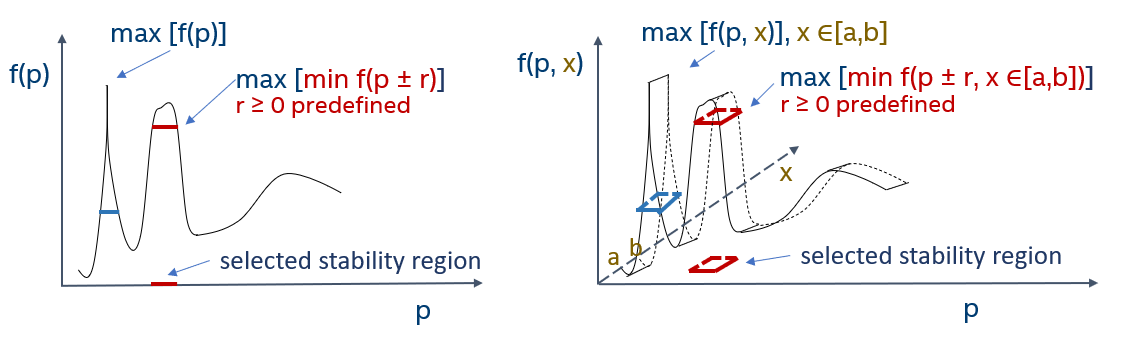
\includegraphics[width= 0.7\columnwidth]{smlp_maxmin.PNG}
\caption{SMLP max-min optimization. On both plots, $p$ denote the knobs. On the right plot we also consider inputs $x$ (which are universally quantified) as part of $f$.} \label{smlp_maxmin}
\end{figure}


The left plot represents optimization problem for $f(p,x)$ when $f$ depends on knobs only (thus $x$ is an empty vector), while the right plot represents the general setting where $x$ is not empty (which is usually not considered in optimization research). In each plot, the blue threshold (in the form of a horizontal bar or a rectangle) denotes the stable maximum around the point where $f$ reaches its (regular) maximum, and the red threshold denotes the stable maximum, which is approximated by our optimization algorithms. In both plots, the regular maximum of $f$ is not stable due to a sharp drop of $f$'s value in the stability region. 
\delete{The right plot depicts the situation when input $x$ ranges in interval $[a, b]$, thus in \emph{max-min} optimization problem, formalized below in Formulas~\eqref{form:opt1}  and  \eqref{form:opt2}, the minimum of $f$ is calculated in the stability region of knobs $p$, with values of $x$ ranging in $[a,b]$.}


%\todozk{In the first formula, in phi condition, should z be y? both are legitimate formulations but b usually refers to model's interface while z represents an optimization threshold?}
%\KK[inline]{ In progress: 
%
%Informally, the  optimization problem is the problem of finding parameters such that an objective function connecting outputs and inputs of the system is near-optimal under  all inputs under the required constraints. Further, in the presence of the stability requirement, the whole region around the solution should also satisfy optimality  constraints.
%
%In the optimization problem we want to find parameters such that output of our system is near-optimal under all constraints.
%
%\[ \regmin{ p}{\theta,\varphi}\coloneqq
    %\min\{f(\vec x'):\vec x'\in  X,\theta(\vec x,\vec x')\} =
%    \mathop{\min\nolimits_{ p'\in X}}\limits_{\theta(p, p')}\varphi(p)
%\text. \]
%
%}

\strut\todozk{remove `near' everywhere}%
Let us first consider optimization without stability or inputs, i.e., far low corner in the exploration cube Figure~\ref{fig:cube}. %\todozk{edge instead of corner?}
%
Given a %binary predicate
formula
%\todofb{Do we need the index $M$ on $\varphi_M$?}%
$\varphi_M$ encoding the model, and an objective function 
$\objv:%
\mathcal{D}_{\mathit{par}}\times
%\mathcal{D}_{\mathit{in}}\times
\mathcal{D}_\mathit{out}\to\mathbb R$, the
%$\objv:\mathcal{D}_\mathit{out}\to\mathbb R$, 
%\todofb{better word for `pure'? Can we re-use terminology from the cube or the intro?}%
standard optimization problem solved by SMLP is stated by Formula~\eqref{form:opt_p}.
%
 \begin{equation}\label{form:opt_p}
 \regmax{\varphi_M}{\objv}
 \eqdef\mathop{\max\limits_{p}} \{z \mid  
    \forall y\changedto[{~(} \varphi_M(p,y)  \implies  
    \objv(p,y) \geq z
    \changedto])\}
\end{equation}
%\todofb{domain of $\objv$ needs changes, they were done in~\ref{note:changes-to-objv}.}%
A solution to this optimization problem %\eqref{form:opt_p}
is the pair $(p^*,\regmax{\varphi_M}{\objv})$, where 
$p^*{}\in\mathcal{D}_{\mathit{par}}$ is a value of parameters $p$ on which the maximum $\regmax{\varphi_M}{\objv}\in\mathbb R$ of the objective function $\objv$ is achieved
for the output $y$ of the model on $p^*$.
In most cases it is not feasible to exactly compute the maximum.
To deal with this, SMLP computes maximum with a specified accuracy. 
Consider $\varepsilon >0$. 
We refer to %\todofb{$\vec x\in X$?}%
values $(\tilde p,\tilde z)$ as a
solution to the optimization problem with
%\old{\todofb{Consider \emph{not} defining `accuracy' $\leadsto$ strengthened notion}}%
\emph{accuracy} $\varepsilon$, or \emph{$\varepsilon$-solution},
if $\tilde z\leq \regmax{ \varphi_M}{\objv}  <\tilde z+\varepsilon$ holds and
%$z^*=%f(\vec x^*)
 %for a solution $p^*$ to \eqref{eq:max-min},
 %and
%$\tilde y=\regmax{\tilde{p}}{\theta,o}$.
%
$\tilde z$ is a lower bound on the objective, i.e., $\forall y [ \varphi_M(p,y)  \implies  
    \objv(p,y) \geq \tilde z] $ holds.


Now, we consider \emph{stable optimized synthesis}, i.e., the top right corner of the exploration cube.
%The problem can be formulated as the following formula \eqref{form:opt1}, expressing maximization of a lower bound  on the objective function over parameters values under GEAR formula constraints
The problem can be formulated as the following Formula~\eqref{form:opt1}, expressing maximization of a lower bound  on the objective function $\objv$ over parameter values under stable synthesis constraints.
%
\begin{equation}\label{form:opt1}
\regmax{\varphi_M}{\objv,\theta}
\eqdef\mathop{\max\limits_{p}} \{z \mid\eta(p) \wedge
    \forall p'~
    \forall x y~[
    \theta(p,p') \implies
    (\varphi_M(p',x,y)  \implies 
     \varphi_{\mathit{cond}}^{\geq}(p',x,y,z))
    ]\}
\end{equation}
where
\[
\varphi_{\mathit{cond}}^{\geq}(p',x,y,z)
\eqdef \alpha(p',x) \implies (\beta(p',x,y) \wedge \objv(p',x,y) \geq z).
\]
%
The stable synthesis constraints are part of a GEAR formula and include usual $\eta, \alpha, \beta$ constraints together with the stability constraints $\theta$.
%
%that bounds over parameter values
%
Equivalently, stable optimized synthesis can be stated as the \emph{max-min} optimization problem, Formula~\eqref{form:opt2}
\begin{equation}\label{form:opt2}
\regmax{\varphi_M}{\objv,\theta}
\eqdef
\mathop{\max\limits_{p}} \mathop{\min\limits_{x, p'}}
\{ z \mid \eta(p) \wedge
    \forall y~[
     \theta(p,p') \implies
     (\varphi_M(p',x,y)  \implies  \varphi_{\mathit{cond}}^{\leq}(p',x,y,z))]\}
\end{equation}
%
%
%     \begin{equation}\label{form:opt}
%   \mathop{\max\limits_{p}} \mathop{\min\limits_{x, p'}\nolimits_{y}}  ~\eta(p) \wedge
%    \forall y'~[
%     \theta(p,p') \wedge \varphi_M(p',x,y')  \implies  \varphi_{\mathit{cond}}(p',x,y') \wedge o(p',x,y')
 %   ]
%\end{equation}
where \[
\varphi_{\mathit{cond}}^{\leq}(p',x,y,z)
\eqdef\alpha(p',x) \implies (\beta(p',x,y) \wedge \objv(p',x,y) \leq z)\text.\]
%\todofb{`The notion of $\varepsilon$-solutions carries over from the standard optimization problem'?}%
In Formula~\eqref{form:opt2} the minimization predicate in the stability region corresponds to the universally quantified $p'$ ranging over this region in~\eqref{form:opt1}.
An advantage of this formulation is that this formula can be adapted to define other aggregation functions over the objective's values on stability region.
For example, that way one can represent the \emph{max-mean} optimization problem, where one wants to maximize the mean value of the function in the stability region rather one the min value (which is maximizing the worst-case value of $f$ in stability region).
Likewise, Formula~\eqref{form:opt2} can be adapted to other interesting statistical properties of distribution of values of $f$ in the stability region.%\footnote{Solving such optimization problems with SMT solver

We can explicitly incorporate assertions in stable optimized synthesis by defining $\beta(p',x,y)\eqdef \beta'(p',x,y) \wedge \assert(p',x,y)$, where  $\assert(p',x,y)$ are assertions required to be valid in the entire stability region around the selected configuration of knobs $p$.
%(So even if the configuration is perturbed within the limits of stability guard $\theta$,
%by the environment or an adversary,
%the configuration will still be
%near-optimal and assertions too will still be valid.)
The notion of $\varepsilon$-solutions for these problems carries over from the one given above for Formula~\eqref{form:opt_p}.

SMLP implements stable optimized synthesis based on the GearOPT$_\delta$ and GearOPT$_\delta$-BO algorithms~\cite{DBLP:conf/fmcad/BrausseKK20,DBLP:conf/ijcai/BrausseKK22}, which are shown to be complete and terminating 
for this problem under mild conditions. 
%
%\todofb{Algorithms also complete under mild conditions}%
These algorithms were further extended in SMLP to Pareto point computations to handle multiple objectives simultaneously.
%\end{comment}





\section{How to run SMLP}\label{sec:run}


Consider a toy dataset in Table~\cref{toy_basic_df} with two inputs $x_1, x_2$, two knobs $i_1, i_2$, and two outputs $y_1, y_2$.
Command to run SMLP in \emph{optimize} mode is given in Figure~\cref{fig:command}.
The optimization problem is specified in the spec file in Figure~\cref{fig:spec}.

\begin{table*}[t]
\centering\small
\begin{tabular}{lrrrrrr}
\hline %\toprule
{} &      x1 &  x2 &    p1 &  p2 &       y1 &       y2 \\
\hline %\midrule
0 &  2.9800 &  -1 &   0.1 &   4 &   5.0233 &   8.0000 \\
1 &  8.5530 &  -1 &   3.9 &   3 &   0.6936 &  12.0200 \\
2 &  0.5580 &   1 &   2.0 &   4 &   0.6882 &   8.1400 \\
3 &  3.8670 &   0 &   1.1 &   3 &   0.2400 &   8.0000 \\
4 & -0.8218 &   0 &   4.0 &   3 &   0.3240 &   8.0000 \\
5 &  5.2520 &   0 &   4.0 &   5 &   6.0300 &   8.0000 \\
6 &  0.2998 &   1 &   7.1 &   6 &   0.9100 &  10.1250 \\
7 &  7.1750 &   1 &   7.0 &   7 &   0.9600 &   1.1200 \\
8 &  9.5460 &   0 &   7.0 &   6 &  10.7007 &   9.5661 \\
9 & -0.4540 &   1 &  10.0 &   7 &   8.7932 &   6.4015 \\
\hline %\bottomrule
\end{tabular}
\caption{Toy dataset $smlp\_toy\_basic.csv$ with two inputs $x_1, x_2$, two knobs $i_1, i_2$, and two outputs $y_1, y_2$.}
\label{toy_basic_df}
\end{table*}

\begin{figure}%[tp]
%\scriptsize
%\tiny
%\small
\begin{verbatim}
 ../src/run_smlp.py -data smlp_toy_basic -out_dir out -pref abc  -mode optimize -pareto t  \
-sat_thresh f -resp y1,y2 -feat x1,x2,p1,p2 -model dt_sklearn -dt_sklearn_max_depth 15 \
-data_scaler min_max -epsilon 0.05 -delta 0.01 -save_model_config f -mrmr_pred 0 -plots f \
-seed 10 -log_time f -spec smlp_toy_basic -pref try
\end{verbatim}
\caption{Example of SMLP's command to build a decision tree model and find .}
\label{fig:command}
\end{figure}



\begin{figure}%[tp]
%\scriptsize
%\tiny
\small
\begin{verbatim}
{
  "version": "1.2",
  "variables": [
    {"label":"y1", "interface":"output", "type":"real"},
    {"label":"y2", "interface":"output", "type":"real"},
    {"label":"x1", "interface":"input", "type":"real", "range":[0,10]},
    {"label":"x2", "interface":"input", "type":"int", "range":[-1,1]},
    {"label":"p1", "interface":"knob", "type":"real", "range":[0,10], "rad-rel":0.1, "grid":[2,4,7]},
    {"label":"p2", "interface":"knob", "type":"int", "range":[3,7], "rad-abs":0.2}
  ],
  "alpha": "p2<5 and x1==10 and x2<12",
  "beta": "y1>=4 and y2>=8",
  "eta": "p1==4 or (p1==8 and p2 > 3)",
  "assertions": {
    "assert1": "(y2**3+p2)/2>6",
    "assert2": "y1>=0",
    "assert3": "y2>0"
  },
  "objectives": {
    "objective1": "(y1+y2)/2",
    "objective2": "y1"
  }
}
\end{verbatim}
\begin{tikzpicture}[remember picture,overlay,shift={(22em,\baselineskip)}]
\node[anchor=south west]{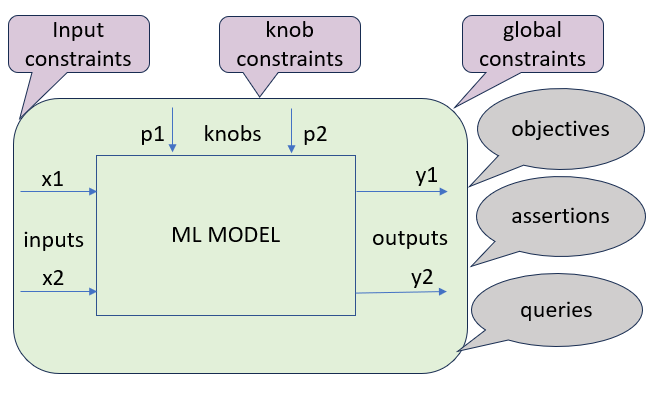
\includegraphics[height=14\baselineskip]{smlp_encoding.PNG}};
\end{tikzpicture}
\vspace*{-1\baselineskip}
\caption{Specification $smlp\_toy\_basic$ used by SMLP command in Figure~\cref{fig:command}.}
\label{fig:spec}
\end{figure}


Optimization progress is reported in  file $try\_smlp\_toy\_basic\_optimization\_progress.csv$, where $try$ is the run ID specified using option '-pref try'; $smlp\_toy\_basic$ is the name of the data file, and $optimization\_progress.csv$ is suffix for that report. More details on input, knob, output and objective values used to prove the upper and lower bounds of the objectives during search for pareto optimum are reported in file $try\_smlp\_toy\_basic\_optimization\_progress.json$. 

\subsection{Design of experiments}\label{sssect:doe}

Most DOE methods
are %mainly
based on understanding multivariate distribution of legal value combinations
of inputs and knobs %, possibly combined with random sampling
in order to sample the system.
\pagebreak[3]
When the number of system inputs and/or knobs is large (say hundreds or more), the DOE may not  generate a high-quality coverage of the system’s behavior to enable training models with high accuracy.
%When the number of system inputs and/or knobs is large (say hundreds or more),
%the DOE methods that are mainly based on understanding multivariate distribution of legal value combinations of inputs and knobs,
%possibly combined with random sampling,
%cannot generate a high-quality coverage of the system's behavior to enable training models with high accuracy.
Model training process itself becomes less manageable when number of input variables grows,
and models are not explainable and thus cannot be trusted.
One way to curb this problem is to select a subset of input features for DOE and for model training.
The problem of combining feature selection with DOE generation and model training
is an important research topic of practical interest,
and SMLP supports multiple practically proven ways
to select subsets of features and feature combinations as inputs to DOE and training,
including the \emph{MRMR} feature selection algorithm~\cite{DBLP:journals/jbcb/DingP05},
and a \emph{Subgroup Discovery (SD)} algorithm~\cite{DBLP:books/mit/fayyadPSU96/Klosgen96,DBLP:conf/pkdd/Wrobel97,DBLP:journals/widm/Atzmueller15}.
The MRMR algorithm selects a subset of features according to the principle of \emph{maximum relevance and minimum redundancy}.
It is widely used for the purpose of selecting a subset of features for building accurate models,
and is therefore useful for selecting a subset of features to be used in DOE;
it is a default choice in SMLP for that usage.
The SD algorithm selects regions in the input space relevant to the response,
using heuristic statistical methods,
and such regions can be prioritized for sampling in DOE algorithms.



\subsection{Root cause analysis}

We view the problem of root cause analysis as dual to the stable optimized synthesis problem: while during optimization with stability we are searching for regions in the input space (or in other words, characterizing those regions) where the system response is good or excellent, the task of root-causing can be seen as searching for regions in the input space where the system response is not good (is unacceptable). Thus simply by swapping the definition of excellent vs unacceptable, we can apply SMLP to explore weaknesses and failing behaviors of the system.

Even if a number of witnesses (counter-examples to an assertion) are available, they represent discrete points in the input space and it is not immediately clear which value assignments to which variables in these witnesses are critical to explain the failures. Root causing capability in SMLP is currently supported through two independent approaches:
a \emph{Subgroup Discovery (SD)} algorithm that searches through the data for the input regions where there is a higher ratio (thus, higher probability) of failure; to be precise, SD algorithms support a variety of \emph{quality functions} which play the role of optimization objectives in the context of optimization.
%\delete{SD and Rule Learning algorithms have been used successfully for root-causing in a number of EDA domains (and beyond).}
To find input regions with high probability of failure, SMLP searches for stable witnesses to failures. These capabilities, together with feature selection algorithms supported in SMLP, enable researchers to develop new root causing capabilities that combine formal methods with statistical methods for root cause analysis. 


\subsection{Model refinement loop}\label{s.refinement}

Support in SMLP for selecting DOE vectors to sample the system and generate a training set was discussed in Subsection~\ref{sssect:doe}.
Initially, when selecting sampling points for the system, it is unknown which regions in the input space are really relevant for the exploration task at hand.
Therefore some DOE algorithms also incorporate random sampling and
sampling based on previous experience and familiarity with the design, such as sampling nominal cases and corner cases, when these are known.
For model exploration tasks supported by SMLP, it is not required to train a model that will be an accurate match to the system everywhere in 
the legal search space of inputs and knobs.
%\todofb{I don't understand what `adequate' means. First time distinguished from `accurate' here.}%
We require to train a model that is an \emph{adequate} representation of the system for the task at hand, 
meaning that the exploration task solved on the model solves this task for the system as well.
Therefore SMLP supports a \emph{targeted model refinement} loop to
enable solving the system exploration tasks by solving these tasks on the model instead.
The idea is as follows: when a stable solution to model exploration task is found, it is usually the case that there are not 
many training data points close to the stability region of that solution.
This implies that there is a high likelihood that the model does not accurately represent the system in the stability region of the solution.
Therefore the system is sampled in the stability region of the solution, and these data samples are added to the initial training data to 
retrain the model and make it more adequate in the stability region of interest.
%Therefore the system is sampled in the stability region of the solution. If the learning is confirmed on the system using these newly 
% vsampled points, then the model exploration goal has been accomplished and model refinement can stop. Otherwise these data samples 
%are added to the initial training data to retrain the model and make it more adequate in the stability region of interest.
Samples in the stability region of interest can also be assigned higher weights compared to other samples to help training to achieve 
higher accuracy in that region. More generally, higher adequacy of the model can be achieved by sampling distributions biased towards 
prioritizing the stability region during model refinement.

%\begin{comment}
\strut\todofb{It is hard to follow the reasoning laid out in these two following paragraphs.}%
Note that model refinement is required only to be able to learn properties on the system by exploring these properties on the model.
As a simple scenario, let us consider that we want to check an assertion $\assert(p,x,y)$ on the system.
If a $\theta$-stable counter example $x^*$ to $\assert(p,x,y)$ for a configuration $p^*$ of knobs exists 
on the model according to Definition~\ref{def:stable:witness:validity} 
(which means that  $x^*$ is a $\theta$-stable witness for query $\query(p^*, x, y) \eqdef \neg \assert(p^*,x,y)$), 
then the system is sampled in the $\theta$--stability region of $p^*$ (possibly with $x^*$ toggled as well in a small region around $x^*$).
If the failure of assertion $\assert(p,x,y)$ is reproduced on the system using the stable witness $x^*$ and a configuration in the $\theta$-stability region of $p^*$,
then the model exploration goal has been accomplished (we found a counter-example to $\assert(p,x,y)$ on the system) and model refinement can stop.
Otherwise the system samples can be used to refine the model in this region.
For that reason, the wider the $\theta$-stability region, the higher the chances to reproduce failure of assertion $\assert(p,x,y)$ on the system.

On the other hand, if the $\assert(p,x,y)$ does not have a $\theta$-stable counter-example, then it is still possible that $\assert$ is not valid on the system 
but it cannot be falsified on the model due to discrepancy between the system and model responses in some (unknown to us) input space.
In this case one can strengthen $\assert(p,x,y)$ to $\assert'(p,x,y)$ (for example, assertion $\assert(p,x,y) \eqdef y \geq 3$ can be 
strengthened to $\assert'(p,x,y) \eqdef y \geq 3.01$),
or one can weaken the stability condition $\theta_r$ to  $\theta_{r'}$ by shrinking the stability radii $r$ to $r'$; or do both.
If the strengthened assertion $\assert'(p,x,y)$ has a $\theta_{r'}$-stable counter-example $x'$ for a configuration $p'$ on the model, 
then $p', x'$ can be used to find a counter-example to the original assertion $\assert(p, x, y)$ on the system in the same way as with $p^*, x^*$ before.
If failure of the original assertion $\assert$ is reproduced on the system, the model refinement loop stops, otherwise it can continue using other 
strengthened versions of the original assertion and or shrinking the  stability radii even further.
Similar reasoning is applied to other modes of design space exploration. In particular, in the optimization modes, one can confirm 
or reject on the system an optimization threshold proved on the model, and in the latter case the model refinement loop 
will be triggered by or providing new data-points 
that can be used for model refinement  in this region, through re-training or incremental training of a new model. 
\KK[inline]{Might be move to the end of 1st para: Similar reasoning is applied to other modes of design space exploration. 
In particular, in the optimization modes, the region around optimal solution can be sampled and simulated by the system, 
and either confirm the model predictions or provide new data-points that can be used for model refinement in this region.}
%\end{comment}

\delete{OLD: 
Usefulness of an ML model is limited by its accuracy with respect to the system that it models.
A major share of the gap between the system response and the model response on same inputs is due to poor quality of training set that was obtained by sampling the system.
SMLP support for selecting DOE vectors to sample the system and generate a training set was discussed in Subsection~\ref{sssect:doe}.
SMLP also supports a \emph{model refinement loop} based on model exploration results in SMLP.
We are interested in \emph{targeted refinement} of the model, in input regions where it matters for the task at hand.
We explain how model refinement works, and relevance of stable witnesses for that goal. The idea is as follows:
Consider a condition of interest, called $query$.
For example, $query$ can be negation of an assertion validity formula
$\forall x y (\varphi_M(p,x,y)  \implies \assert(p,x,y))$
that is expected to be valid on the system, say
$query_1 \equiv \exists x. y < 3$ where $assert(p,x,y) \equiv y \geq 3$,
%$query_1 \equiv \neg\operatorname{assert}(x, y)\equiv \neg (y \geq 3)$, 
or an optimization threshold query
$\forall x y (\varphi_M(p,x,y)  \implies \assert(p,x,y))$
for an objective $o$ to optimize,
say $query_2\equiv o \geq 5$,
under model constraints $\varphi_M(x,y)$.
If a stable witness to this query exists on the model,
one samples the system in the stability region of that witness.
If one of these data samples is a witness to that query on the system,
then querying the model helped us to find a witness to the query on the system.
(If that query was $query_1$, this way we have found a real violation of
$\operatorname{assert}(x,y)$ on the system;
and if that query was $query_2$,
we have confirmed the objective threshold $o \geq 5$ on the system.)
If on the other hand none of the newly sampled data points (including the witness itself) is a witness of $query$ on the system,
we have discovered \changed{a} discrepancy between the model and system response in the input region of interest (relevant to that query of interest),
and the newly sampled data points can be added to the training data and model re-trained,
to improve its quality in the stability region of interest.
Note that $query$ can also be negation of a strengthened assertion
(say assertion $y \geq 3$ can be strengthened to $y \geq 3.001$)
and thereby weaken the query,
and even if the original query does not have a stable witness, the modified one might have,
and a stable witness to the modified query can be used in model refinement or
finding a bug on the system
in the same way as a witness to the original query if it existed.
Thus\changed{, the} model refinement loop also works when all assertions of interest are valid on the model.
}


\delete{

\section{MRC usage}\label{sec:mrc}

Quick command template for solving the MRC problem on a single machine:
\begin{equation}
\cmdline{\progmrc{} -i \emph{data.csv} -s \emph{data.spec} -t \emph{target/dir} -j 112 run}
\tag{$*$}\label{cmd:mrc}
\end{equation}
Here, \file{\emph{data.csv}} is the data set containing training samples,
\file{\emph{data.spec}} is the specification file detailed in \cref{sec:.spec}\todo{add example in release or documentation},
\cmdstyle{-t \emph{target/dir}} is an optional working directory for the prover and \cmdstyle{-j 112} is the maximum number of parallel jobs to run.

For each combination of categorical parameters \literal{CH} and \literal{Byte}s the tool: 
\begin{enumerate}
\item builds a NN model representing the target function,
\item computes thresholds and safe and stable regions for these representation,
\item extends regions and thresholds to other bytes in the channel.
\end{enumerate}

The output will be a file \file{\emph{target/dir}/rank0/shared1.csv} containing
the safe and stable regions and thresholds across all \literal{Byte}s for each
\literal{CH}.
%, see also \cref{sec:mrc-def}.
\todo{output format/values/meaning}

For details, please see the following sections.


\subsection{Problem definition}\label{sec:mrc-def}
Assume a data set containing, besides other integer or floating-point features,
the categorical input features \literal{Byte},
\literal{CH} and \literal{RANK} ranging over
$\{\literal0,\literal1,\literal2,\literal3,\literal4,\literal5,\literal6,\literal7\}$,
$\{\literal0,\literal1\}$ and $\{\literal0\}$, respectively,
is described in the CSV file \file{data.csv}. Furthermore, assume the codomain
is labelled \literal{delta}.

The goal is to find, for each \literal{Byte} and \literal{CH},
\begin{enumerate}
\def\labelenumi{(\alph{enumi})}
\item a threshold $t$ among $\{0.05\cdot i:i=0,\ldots,20\}$ for which safe
	regions exist,
\item $n\leq 100$ safe regions $R_1,R_2,\ldots,R_n$, which satisfy the .spec and
\item thresholds for all $R_i$ among $\{0.05\cdot i:i=0,\ldots,20\}$ for the
	other \literal{Byte}s in this \literal{CH}.
\end{enumerate}
The data instances $(I^{c,b},\mathcal D^{c,b})$ with
$I^{c,b}=(N^{c,b},\mathcal N_D^{c,b},o,\mathcal N_o^c)$
defining the target function $f_{I^{c,b},\mathcal D^{c,b}}$ for which the
above thresholds should hold is defined for each \literal{CH}/\literal{Byte}
combination $(c,b)$ by
\begin{itemize}
\item the .spec file \file{data.spec} defining the domain $D$
	and the finite set of regions, see \cref{sec:.spec}, and
\item the data set
	%$\bigcup_{c\in\{0,1\}}\bigcup_{b\in\{0,\ldots,7\}}\mathcal D^{c,b}$
	described by the CSV file \file{data.csv}, where
	the restriction and projection to $(c,b)$, $\mathcal D^{c,b}$,
	is a subset of the domain $D$
\end{itemize}
in the following way:
\begin{itemize}
\item
	The NN $N^{c,b}$ is defined by the training algorithm on
	$\mathcal D^{c,b}$.
\item
	The data normalization $\mathcal N_D^{c,b}$ corresponds to the pair of
	normalization $N_{D,\mathrm i}^{c,b}=\operatorname{norm}_{I^{c,b}}$
	and denormalization
	$N_{D,\mathrm o}^{c,b}=\operatorname{norm}_{J^{c,b}}^{-1}$ where
	$\operatorname{norm}_{[\vec a,\vec b]}:\vec x\mapsto ((x_i-a_i)/(b_i-a_i))_i$
	is the component-wise normalization to domain bounds $I^{c,b}$
	defined by $\mathcal D^{c,b}$
	and $\operatorname{norm}_{J^{c,b}}^{-1}$ is the inverse of
	$\operatorname{norm}_{J^{c,b}}$
	where $J^{c,b}$ are the codomain bounds defined by $\mathcal D^{c,b}$.

	This definition assumes $I^{c,b}$ and $J^{c,b}$ do not contain
	point intervals.
\item
	Objective funtion $o$ is the projection to the first component
	\literal{delta} (i.e.\ the identity).
\item
	The objective normalization $\mathcal N_o^c=\operatorname{norm}_{C_c}$
	is shared across all $b$ per $c$ and defined on the bounds $C_c$ of the
	objective function $o$ on $\bigcup_{b\in\{0,\ldots,7\}}\mathcal D_{c,b}$
	projected to the codomain.
\end{itemize}

By the above definition, the entries besides
\literal{"obj-bounds"} and \literal{"train"}
in the derived instance description file
\file{\emph{target/dir}/rank0/ch\{0,1\}/byte/\{0..7\}/model\_gen\_*\_12.json}
(see \cref{sec:.gen} for details) are fixed.
It should have the following form:
\begin{quote}\footnotesize\color{\literalColor}\begin{verbatim}
{
   "obj-bounds" : {
      "max" : 68,
      "min" : -57.6
   },
   "objective" : "delta",
   "pp" : {
      "features" : "min-max",
      "response" : "min-max"
   },
   "response" : [
      "delta"
   ],
   "train" : {
      "activation" : "relu",
      "batch-size" : 32,
      "epochs" : 30,
      "optimizer" : "adam",
      "seed" : 1234,
      "split-test" : 0.2
   }
}
\end{verbatim}\end{quote}


\subsection{How to use \SolverAbbrv to solve the MRC problem}

The following steps are performed during the run of \SolverAbbrv on the MRC
problem when the command \eqref{cmd:mrc}  given at the beginning of
\cref{sec:mrc}, is invoked. We assume that the user provided a specification
file \file{data.spec} and training data set in the file \file{data.csv}.
Although the system does not require futher interaction we give commands that
can be performed to execute the corresponding steps separately  (and its
dependencies) here as well.

%problem for the version of \Solver described here.
%The following steps are required to solve the MRC problem for the version of
%\Solver described here.
%Though steps corresponding to \cref{step:shai:2,step:shai:3,step:shai:4,step:shai:5} can
%be performed automatically by invoking
%the command \eqref{cmd:mrc} given at the beginning of \cref{sec:mrc},
%we also give the concrete commands to just perform the
%corresponding step (and its dependencies) here as well.
\begin{enumerate}
%\item\label{step:shai:1}
%	Write a specification file \file{data.spec}.
\item\label{step:shai:2}
	Split the data set into $2\cdot8$ data sets and set up the corresponding
	subdirectories \file{rank0/ch$c$/byte/$b$/} for the next steps,
	one for each combination $(c,b)$ of \literal{CH} and \literal{Byte}.

	\cmdline{\progmrc{} -i \emph{data.csv} -s \emph{data.spec}
		-t \emph{target/dir}
		run prepare}

	resulting in a directory tree at \emph{\file{target/dir}} prepared for
	the following steps.
\item\label{step:shai:3}
	Train NNs for all $(c,b)$.

	In \file{\emph{target/dir}}: \cmdline{\progmrc{} -j 16 run train}
\item\label{step:shai:4}
	Find thresholds and safe regions for each $(c,b)$.

	In \file{\emph{target/dir}}: \cmdline{\progmrc{} -j 16 run search}
\item\label{step:shai:5}
	For each $c$, determine thresholds of $R$ for $(c,b')$
	for each $R,b,b'$ where $b'\neq b$ and $R$ has been found safe for
	$(c,b)$ in \cref{step:shai:4} and
%\item
	collect results into \file{shared1.csv}.

	In \file{\emph{target/dir}}: \cmdline{\progmrc{} -j 112 run collect}
\end{enumerate}
Each of these steps depends on the previous.
%The only step to be performed manually is \cref{step:shai:1}.
The parameter \cmdstyle{-j \emph N} in the above commands is optional and
denotes the maximum number of parallel jobs to use. The values \cmdstyle{\emph N}
given above are the maximum bounds on the number of parallel jobs that
-- given enough resources -- may provide a noticable speedup of the entire
computation.


\subsection{Internals and control files for the MRC instance}
In order to change defaults for various settings, we briefly describe the
important configuration files as set up by the \cmdstyle{prepare} stage of
\cmd{\progmrc} and how the solver invocations for multiple \literal{CH} and
\literal{Byte} combinations are performed.

The parallel execution of the steps in
\cref{step:shai:3,step:shai:4,step:shai:5} of the previous section
is delegated to \cmd{make} by means of the
following \file{Makefile}s generated by \cref{step:shai:2} in
\emph{\file{target/dir}}:
\begin{enumerate}
\item\label{mk:rank} \file{rank0/Makefile}

	Entry point; delegation to \cref{mk:byte} for \cmd{make} targets
	\cmdstyle{train} and \cmdstyle{search}.
	Delegates to \cref{mk:ch} for the \cmdstyle{collect} target and
	generates the result file \file{rank0/shared1.csv}.

\item\label{mk:ch} \file{rank0/ch\{0,1\}/Makefile}

	Delegates \cref{mk:byte} for the \cmdstyle{collect} target,
	synchronizes the computations of the shared safe regions and
	collects the results in \file{rank0/ch\{0,1\}/shared1.csv}.

\item\label{mk:byte} \file{rank0/ch\{0,1\}/byte/\{0..7\}/Makefile}

	Main driver: Runs the search for a specific $(c,b)$ combination either
	with (for the \cmdstyle{collect} target in \cref{mk:rank}) or without
	(for the \cmdstyle{search} target in \cref{mk:rank}) by taking into
	account customizations defined in the \file{params.mk} files in the
	following paths under \emph{\file{target/dir}} as well as
	\file{src/defaults.mk} and \file{src/scripts.mk}.
	Each \file{params.mk} above one in a subdirectory gives defaults for
	the latter.

	\begin{itemize}
	\item\file{params.mk}
	\item\file{rank0/params.mk}
	\item\file{rank0/ch\{0,1\}/params.mk}
	\item\file{rank0/ch\{0,1\}/byte/\{0..7\}/params.mk}
	\end{itemize}

	As generated by the \cmdstyle{prepare} stage of \cmd{\progmrc},
	all but the top-level \file{params.mk} just delegate to the one
	immediately above. The top-level one maintains defaults for the MRC
	application, such as defining $N_o$ and the specific \cmd{make} targets
	for computing shared regions across one \literal{CH}.

	The template used by the \cmdstyle{prepare} stage for the top-level file
	can be found in \file{src/mrc-params.mk} while the remaining ones are
	generated. %by \cmd{src/split-categorical2.py} which is called indirectly.

	\file{rank0/ch\{0,1\}/byte/\{0..7\}/Makefile} is a symlink to the
	template \file{src/datasets.mk} distributed with \SolverAbbrv and
	created in the \cmdstyle{prepare} stage.
\end{enumerate}


\subsection{MRC options}
\begin{cmdhelp}\begin{verbatim}
smlp-mrc.sh [-OPTS] COMMAND [ARGS...]

Common options [defaults]:
  -d           debug this script
  -h           print this help message
  -k           keep created files / directories on errors
  -j JOBS      run N jobs in parallel; if JOBS is 0 determine via lscpu(1) [1]
  -t TGT       path to target instance directory [derived from basename of SRC
               if given, otherwise '.']

Options used by 'prepare' stage:
  -i SRC       path to source data set ending in .csv
  -s SPEC      path to .spec file describing the target instance

Options used by 'train' stage [defaults replicated from src/defaults.mk]:
  -b BATCH     batch size [32]
  -e EPOCHS    number of epochs to use for training [30]
  -f FILTER    percentile of lowest OBJT values to ignore for training [0]
  -l LAYERS    layer specification [2,1]
  -o OBJT      objective function [RESP]
  -r RESP      response features [delta]
  -s SEED      random number seed for numpy and tensorflow [1234]

Options used by 'search' and 'collect' stages
[defaults replicated from src/defaults.mk]:
  -c COFF      center threshold offset from threshold [0.05]
  -n N         restrict to maximum of N safe regions [100]
  -L TLO       minimum threshold to consider [0.00]
  -H THI       maximum threshold to consider [0.90]

Commands [defaults]:
  run [STAGE]  execute all stages up to STAGE [collect]

Stages (in dependency order):
  prepare      use SRC to setup a fresh TGT instance
  train        train NN models according to prepared TGT instance
  search       determine safety thresholds for TGT instance
  collect      collect shared safe regions
\end{verbatim}\end{cmdhelp}





\section{Components}

%Due to the current version of \Solver being the result of general research into
%the problem, automation has not been the priority.
This section provides an
overview of the individual components involved in the use cases described in
\cref{sec:mrc}, gives an overview of the full functionality as implemented
in the current version and provides details about the .spec file and
the derived instance description.

\subsection{Introduction}
The tools distributed in \SolverAbbrv can be used stand-alone to solve a
specific problem. However, in order to find thresholds for the existence of safe
regions, that is, solving the discretized optimization problem
\[ \max\{t\in\{t_1,\ldots,t_n\}\mid \exists R.\,R~\text{is safe wrt.}~t\} \]
in addition to determining
\[ t_{R,I}=\max\{t\in\{t_1,\ldots,t_n\}\mid R~\text{is safe wrt.}~t~\text{in}~I\} \]
for given regions $R$ and multiple instances $I$,
the wrapper script \cmd{\progmrc} along with default \cmd{make} template
files specifically tailored for the MRC problem are included.
The MRC problem is defined in detail in \cref{sec:mrc}.

The core solver is \cmd{src/\provenn}. It has many options regarding
specific search strategies, domain grids, bounds modifying the target function
as well as other heuristics. Details can be found in \cref{sec:nn_model2.py}.

The program \cmd{src/\trainnn} takes care of training NNs on data
sets and writing information about domain- and codomain-normalization, the
correspondence between NN output(s) and the data set's features as well as
the objective function and bounds into the files \file{data\_bounds\_*\_12.json}
(containing only the features' bounds) and \file{model\_gen\_*\_12.json}
(containing the remaining parameters, called derived instance description).

The version of \SolverAbbrv described here is referred to as \SolverVersion.


\subsection{Specification file}\label{sec:.spec}
Specification file contains description of the domain of the target function, which  can also include domain grid. 

%All tools operating on the grid or domain require at least a specification
%(.spec file), usually called \file{data.spec}.
It is used to define the domain of the target function, the radii of the
regions under consideration and the quantification over the domain.

The specification file format and its correspondence to domain and regions is
described in \file{doc/spec.pdf} and subject to change.


\subsection{Derived instance description}\label{sec:.gen}
The derived instance description file usually called
\file{model\_gen\_data\_12.json} contains a JSON object with at least
the following entries. It can be generated by
\cmd{src/\trainnn}.
\begin{description}
\item[\literal{"obj-bounds"}:]
	Numeric entries in a sub-object under keys \literal{"min"} and
	\literal{"max"} defining the bounds on the objective function on the
	data set used for training.
\item[\literal{"objective"}:]
	A string of one of the following patterns describing the form of the
	objective function to be applied to the output of the NN.
	\begin{itemize}
	\item\literal{"\emph{feature}"}:
		projection to \literal{\emph{feature}}, e.g. \literal{"delta"}.
	\item\literal{"\emph{feature$_1$}-\emph{feature$_2$}"}:
		projection to \literal{\emph{feature$_1$}} minus the
		projection to \literal{\emph{feature$_2$}}; e.g.
		\literal{"Up-Down"}.
	\end{itemize}
\item[\literal{"pp"}:]
	Sub-object containing information about data normalization
	(pre-/postprocessing) for values in the domain (\literal{"features"})
	and codomain (\literal{"response"}), each taking either the string
	\literal{"min-max"} for normalization based on bounds in the file
	\file{data\_bounds\_*\_12.json} or \literal{null} for no normalization.
\item[\literal{"response"}:]
	An ordered list containing the feature labels corresponding to
	\literal{"type": "response"} objects in the .spec file.
\end{description}
The object may optionally contain parameters used for training the NN model under
the key \literal{"train"}.


\subsection{Training NNs}
Performed by \cmd{src/\trainnn}, which has the following options:
\begin{cmdhelp}\begin{verbatim}
usage: src/train-nn.py [-h] [-a ACT] [-b BATCH] [-B BOUNDS] [-c [CHKPT]]
                       [-e EPOCHS] [-f FILTER] [-l LAYERS] [-o OPT]
                       [-O OBJECTIVE] [-p PP] [-r RESPONSE] [-R SEED] -s SPEC
                       [-S SPLIT]
                       DATA

positional arguments:
  DATA                  Path excluding the .csv suffix to input data file
                        containing labels

optional arguments:
  -h, --help            show this help message and exit
  -a ACT, --nn_activation ACT
                        activation for NN [default: relu]
  -b BATCH, --nn_batch_size BATCH
                        batch_size for NN [default: 200]
  -B BOUNDS, --bounds BOUNDS
                        Path to pre-computed bounds.csv
  -c [CHKPT], --chkpt [CHKPT]
                        save model checkpoints after each epoch; optionally
                        use CHKPT as path, can contain named formatting
                        options "{ID:FMT}" where ID is one of: 'epoch', 'acc',
                        'loss', 'val_loss'; if these are missing only the best
                        model will be saved [default: no, otherwise if CHKPT
                        is missing: model_checkpoint_DATA.h5]
  -e EPOCHS, --nn_epochs EPOCHS
                        epochs for NN [default: 2000]
  -f FILTER, --filter FILTER
                        filter data set to rows satisfying RESPONSE >=
                        quantile(FILTER) [default: no]
  -l LAYERS, --nn_layers LAYERS
                        specify number and sizes of the hidden layers of the
                        NN as non-empty colon-separated list of positive
                        fractions in the number of input features in, e.g.
                        "1:0.5:0.25" means 3 layers: first of input size,
                        second of half input size, third of quarter input
                        size; [default: 1 (one hidden layer of size exactly
                        #input-features)]
  -o OPT, --nn_optimizer OPT
                        optimizer for NN [default: adam]
  -O OBJECTIVE, --objective OBJECTIVE
                        Objective function in terms of labelled outputs
                        [default: RESPONSE if it is a single variable]
  -p PP, --preprocess PP
                        preprocess data using "std, "min-max", "max-abs" or
                        "none" scalers. PP can optionally contain a prefix
                        "F=" where F denotes a feature of the input data by
                        column index (0-based) or by column header. If the
                        prefix is absent, the selected scaler will be applied
                        to all features. This parameter can be given multiple
                        times. [default: min-max]
  -r RESPONSE, --response RESPONSE
                        comma-separated names of the response variables
                        [default: taken from SPEC, where "type" is "response"]
  -R SEED, --seed SEED  Initial random seed
  -s SPEC, --spec SPEC  .spec file
  -S SPLIT, --split-test SPLIT
                        Fraction in (0,1) of data samples to split from
                        training data for testing [default: 0.2]
\end{verbatim}\end{cmdhelp}

\subsection{General safety thresholds}\label{sec:nn_model2.py}
Performed by \cmd{src/\provenn} optionally with the help of
\cmd{src/libcheck-data.so}, which has these options:
\begin{cmdhelp}\begin{verbatim}
usage: src/prove-nn.py [-h] [-b [BOUNDS]] [-B DBOUNDS] [-C CHECK_SAFE]
                       [-d DATA] -g MODEL_GEN [-G GRID] [-n N] [-N]
                       [-o OUTPUT] [-O OBJECTIVE] [-r RESPONSE_BOUNDS] -s SPEC
                       [-S SAFE] [-t THRESHOLD] [-T SAFE_THRESHOLD]
                       [-U CENTER_OFFSET] [-v] [-x TRACE] [-X]
                       NN_MODEL

positional arguments:
  NN_MODEL              Path to NN model in .h5 format

optional arguments:
  -h, --help            show this help message and exit
  -b [BOUNDS], --bounds [BOUNDS]
                        bound variables [default: none; otherwise, if BOUNDS
                        is missing, 0]
  -B DBOUNDS, --data-bounds DBOUNDS
                        path to data_bounds file to amend the bounds
                        determined from SPEC
  -C CHECK_SAFE, --check-safe CHECK_SAFE
                        Number of random samples to check for each SAFE config
                        found [default: 1000]
  -d DATA, --data DATA  path to DATA.csv; check DATA for counter-examples to
                        found regions
  -g MODEL_GEN, --model-gen MODEL_GEN
                        the model_gen*.json file containing the training /
                        preprocessing parameters
  -G GRID, --grid GRID  Path to grid.istar file
  -n N                  number of safe regions to generate in total (that is,
                        including those already in SAFE) [default: 1]
  -N, --no-exists       only check GRID, no solving of existential part
  -o OUTPUT, --output OUTPUT
                        Path to output .smt2 instance [default: none]
  -O OBJECTIVE, --objective OBJECTIVE
                        Objective function in terms of labelled outputs
                        [default: "delta"]
  -r RESPONSE_BOUNDS, --response-bounds RESPONSE_BOUNDS
                        Path to bounds.csv for response bounds to interpret T
                        and ST in [default: use DATA_BOUNDS]
  -s SPEC, --spec SPEC  Path to JSON spec of input features
  -S SAFE, --safe SAFE  Path to output found safe configurations to as CSV
  -t THRESHOLD, --threshold THRESHOLD
                        Threshold to restrict output feature to be larger-
                        equal than [default: search in 0.05 grid between 0 and
                        0.95]
  -T SAFE_THRESHOLD, --safe_threshold SAFE_THRESHOLD
                        Center threshold [default: THRESHOLD+SAFE_OFFSET].
                        Overrides any SAFE_OFFSET.
  -U CENTER_OFFSET, --center_offset CENTER_OFFSET
                        Center threshold offset of threshold [default: 0]
  -v, --verbose         Increase verbosity
  -x TRACE, --trace-exclude TRACE
                        exclude all unsafe i* from trace file
  -X, --trace-exclude-safe
                        exclude also found safe i* from the trace file
\end{verbatim}\end{cmdhelp}


\subsection{Safety thresholds for concrete regions}
Performed by \cmd{src/\provenn} optionally with the help of
\cmd{src/libcheck-data.so}, by passing parameters
\cmdstyle{-NG \emph{path/to/safe/regions.csv}} set via
\begin{quote}
	\file{\emph{target/dir}/rank0/ch\{0,1\}/byte/\{0..7\}/lock.mk}
\end{quote}
which is generated at the end of the \cmdstyle{search} stage.

\subsection{Helper modules}
\subsubsection{\file{libcheck-data.so}}
C-library with Python wrapper defined in \file{checkdata.py} allowing to find
points in the data set within regions defined in the .spec file fast.

\subsubsection{\cmd{split-categorical2.py}}
Helper script for preparing the directory structure according to the MRC
application.

\subsubsection{\cmd{filter-trace.sh}}
Shell script for processing trace files into a more human-readable format by
filtering out non-SMT-related steps and displaying rational solutions as
decimal float approximations.

} % end of delete macro


\bibliography{bib}

\delete{
\begin{thebibliography}{99}
\bibitem{BKK20}
 F. Brauße, Z. Khasidashvili and K. Korovin.
\newblock{Selecting Stable Safe Configurations for Systems Modelled by Neural Networks with ReLU Activation.}
\newblock{2020 Formal Methods in Computer Aided Design, FMCAD 2020}
\newblock{IEEE, 2020}.

\bibitem{BKK22}
 F. Brauße, Z. Khasidashvili and K. Korovin.
\newblock{Combining Constraint Solving and Bayesian Techniques for System Optimization.}  
\newblock{31st International Joint Conference on Artificial Intelligence and the 25th European Conference on Artificial Intelligence, IJCAI-ECAI'22 2022.}


\bibitem{BKK24}
 F. Brauße, Z. Khasidashvili and K. Korovin.
\newblock{SMLP: Symbolic Machine Learning Prover.}
\newblock{Report arXiv: 2402.01415 , 2024.}
\end{thebibliography}
}

\appendix
\section{Concrete Formats}
\subsection{CSV}\label{sec:csv}
A structured line-based text format where the first line describes a
list of column headers and each line after it describes a list the
values corresponding to the respective column in the data set.
A line describes a list of elements $(e_i)_{i=1}^n$, if it corresponds
to the concatenation
$s(e_1)\literal,s(e_2)\literal,\ldots\literal,s(e_n)$
where $s(v)$ is the ASCII representation of $v$.

The list of column headers shall not contain duplicates.
The ASCII representation of ASCII strings made up of printable
characters excluding ``\literal,'' is the identity.
Floating point approximations are represented as the decimal encoding
where ``\literal.'' is the separator between integer and fractional
part. Rational numbers $\frac pq$ are represented by $s(p)\literal/s(q)$
where $s(z)$ is the decimal encoding of $|z|$ prefixed by ``\literal-''
if $z\in\mathbb Z$ is negative.



\end{document}
